\chapter{Wymagania}

\section{Diagram kontekstu}
\begin{figure}[h!]
    \centering
    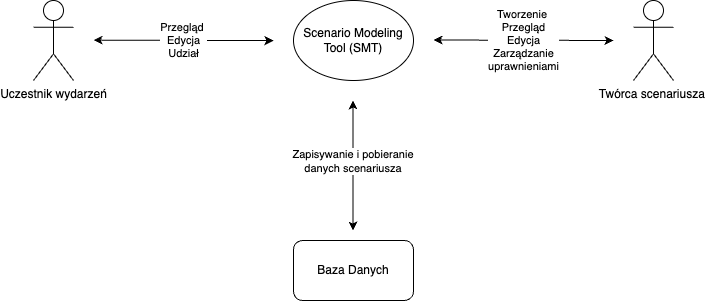
\includegraphics[width=0.99\textwidth]{resources/local/diagram-kontekstu.png}
    \caption{Diagram kontekstu}
\end{figure}

\section{Aktorzy}

\subsection{Twórca scenariusza}
Twórca scenariusza to osoba, która jest odpowiedzialna za tworzenie scenariuszy i ich modyfikowanie oraz dostosowywanie. Ma on możliwość
definiowania wątków, obiektów, typów obiektów, szablonów, asocjacji, a także faz scenariusza w zależności od potrzeb i wymagań. Twórca scenariuszy może również
nadawać uprawnienia edycji lub podglądu innym użytkownikom.

\subsection{Uczestnik wydarzeń}
Uczestnik wydarzeń to osoba biorąca udział w ćwiczeniach. Otrzymuje on dostęp do przeglądania lub modyfikacji scenariusza, w zależności od nadanych uprawnień.
Dzięki temu podziałowi system jest odporny na wszelkie próby naruszenia integralności danych.

\section{Obiekty biznesowe}

\subsection{Organizacja scenariusza}
Scenariusz składa się m.in. z wątków oraz akcji. Każdy wątek jest pewną sekwencją zdarzeń, która może łączyć się z innymi wątkami operacją JOIN, lub dzielić się na wiele wątków operacją FORK.
Kolejnymi składowymi są akcje, które są pojedynczymi punktami w czasie. Dzięki nim użytkownik może zmieniać atrybuty obiektów lub ich asocjacji.

\subsection{Obiekty}
Obiekt jest podstawową jednostką w scenariuszu. Każdy obiekt posiada zestaw atrybutów, które są możliwe do modyfikacji w czasie trwania scenariusza podczas trwania akcji.
Transfer obiektów pomiędzy wątkami jest możliwy tylko dla operacji JOIN lub FORK dla akcji. Obiekty mogą być globalne lub lokalne.

\subsection{Typy}
Typy dzielimy na typy obiektów oraz typy asocjacji. Każdy z nich określa podstawowe cechy charakterystyczne obiektów lub asocjacji na podstawie przypisanego typu.
Typ obiektu określa dostępność globalną między wątkami, kolor, tytuł, a także rodzica w celu zachowania hierarchii. Natomiast typ asocjacji odpowiada za przypisanie odpowiednich typów obiektów do asocjacji oraz weryfikuje poprawność oraz hierarchiczność każdej asocjacji.

\subsection{Szablony}
W systemie możemy wyszczególnić szablon obiektów oraz szablon atrybutów. są one fundamentem, na którym zbudowane są obiekty naszej aplikacji.
Każdy obiekt może być tworzony na podstawie podstawowych wartości zdefiniowanych w szablonie, co niweluje konieczność ręcznego wprowadzania danych obiektu, przy każdym jego dodawaniu.

\subsection{Asocjacje}
Asocjacja jest relacją pomiędzy dwoma obiektami, która jest tworzona i modyfikowana tylko w kontekście wydarzeń. Asocjacje mogą mieć różne typy określające pewne reguły oraz relacje m.in. INSERT lub DELETE.
Każda z asocjacji musi być zgodna z regułami wynikającymi z typów asocjacji.

\subsection{Atrybuty}
Atrybuty są cechami opisującymi dany obiekt. Mogą one być modyfikowane wyłącznie akcji.

\subsection{Wątki}
Wątki są kluczową składową scenariusza, która reprezentuje sekwencję akcji. Każda akcja reprezentuje dane wydarzenie w scenariuszu takie jak zmiana atrybutów lub asocjacji. Dzielą się one na typy:
\begin{enumerate}
\item {START} - rozpoczyna wątek oraz umożliwia dodanie lokalnych obiektów,
\item {END} - kończy wątek,
\item {NORMAL} - jest to standardowa akcja w wątku,
\item {GLOBAL} - określa akcję w wątku globalnym, której zmiany mają priorytet nad typem NORMAL,
\item {JOIN\_IN/JOIN\_OUT} - akcja oznaczająca łączenie wątków,
\item {FORK\_IN/FORK\_OUT} - akcja oznaczająca podział wątku,
\item {IDLE} - akcja pusta, nieposiadająca zmian.
\end{enumerate}
Wątki mogą się łączyć w jedną ścieżkę operacją JOIN lub dzielić operacją FORK. Tylko podczas
trwania tych operacji obiekty mogą być przenoszone pomiędzy wątki. Obiekty globalne są natomiast dostępne w każdym z wątków.

\newpage
\section{Diagram przypadków użycia}
\begin{figure}[h!]
    \centering
    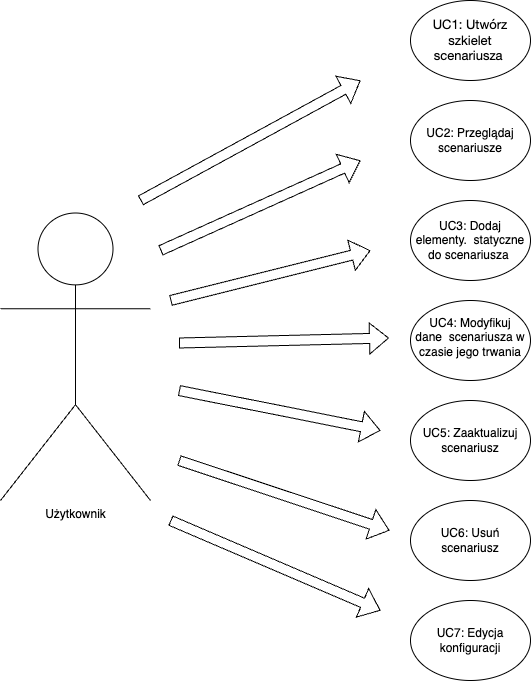
\includegraphics[width=0.8\textwidth]{resources/local/use-case-diagram.png}
    \caption{Diagram przypadków użycia}
    \label{fig:use_case_diagram}
\end{figure}

\section{Tabela przypadków użycia}
\small{
\begin{longtable}{|p{1cm}|p{4.5cm}|p{8cm}|}
    \hline
    \textbf{ID} & \textbf{Przypadek użycia} & \textbf{Opis} \\
    \hline
    \endfirsthead
    \caption[]{Tabela przypadków użycia -- ciąg dalszy} \\
    \hline
    \textbf{ID} & \textbf{Przypadek użycia} & \textbf{Opis} \\
    \hline
    \endhead
    \hline
    \endfoot
    \hline
    \caption{Tabela przypadków użycia} \label{tab:use_case_table} \\
    \endlastfoot
    UC1 & Utwórz szkielet scenariusza & Użytkownik tworzy scenariusz podając jego czas wraz z pozostałymi właściwościami go opisującymi. System dodaje nowy scenariusz wraz z domyślnymi danymi tworzonymi dla nowego scenariusza. \\
    \hline
    UC2 & Przeglądaj scenariusze & Użytkownik przegląda listę dostępnych scenariuszy, z opcją filtrowania, która umożliwia wybranie konkretnego scenariusza oraz jego edycję lub usunięcie. \\
    \hline
    UC3.1 & Utwórz szablon obiektu & Użytkownik tworzy szablon obiektu dostępny we wszystkich scenariuszach. \\
    \hline
    UC3.3 & Utwórz obiekt & Użytkownik tworzy konkretny obiekt przypisany do scenariusza. \\
    \hline
    UC3.4 & Utwórz szablon atrybutu & Użytkownik tworzy szablon atrybutu przyporządkowany do danego szablonu obiektu. \\
    \hline
    UC3.5 & Utwórz atrybut & Użytkownik tworzy atrybut dla konkretnego obiektu. \\
    \hline
    UC3.2 & Utwórz typ obiektu & Użytkownik tworzy typ obiektu dostępny we wszystkich scenariuszach. \\
    \hline
    UC3.6 & Utwórz typ asocjacji & Użytkownik tworzy typ asocjacji dostępny we wszystkich scenariuszach. \\
    \hline
    UC3.7 & Utwórz asocjację & Użytkownik tworzy asocjację pomiędzy dwoma obiektami z danego scenariusza. \\
    \hline
    UC4.1 & Utwórz wątek & Użytkownik tworzy nowy wątek poprzez rozdzielenie wątku istniejącego lub dodanie nowego osobnego wątku. \\
    \hline
    UC4.2 & Utwórz zdarzenie & Użytkownik tworzy zdarzenie wraz ze zdefiniowaniem zmian w asocjacjach lub atrybutach obiektów. \\
    \hline
    UC5.1 & Edycja danych podanych przy tworzeniu scenariusza & Użytkownik modyfikuje właściwości scenariusza podane podczas jego tworzenia. \\
    \hline
    UC5.2 & Edycja elementów statycznych oraz zdarzeń & Użytkownik modyfikuje istniejące elementy statyczne (np. obiekty, atrybuty) wraz z właściwościami zdarzeń i wątków. \\
    \hline
    UC.6 & Usuń scenariusz & Użytkownik usuwa scenariusz po jego wybraniu z listy. System pyta o potwierdzenie i usuwa scenariusz wraz z danymi prywatnymi dla scenariusza na stałe. \\
    \hline
    UC.7 & Edycja konfiguracji & Użytkownik edytuje konfigurację. System wykorzystuje zdefiniowane właściwości przy tworzeniu nowego scenariusza. \\
    \hline
\end{longtable}
}
\normalsize
\section{Wymagania pozafunkcjonalne}
Wymagania pozafunkcjonalne są zgodne ze standardem ISO 25010, zdefiniowanym w książce 
\emph{Systems and Software Engineering — Systems and Software Quality Requirements and Evaluation (SQuaRE) — System and Software Quality Models} 
\cite{iso25010} i zostały opisane w poniższej tabeli:

\section{Tabela wymagań pozafunkcjonalnych}
\small{
\begin{longtable}{|p{1cm}|p{2.5cm}|p{4.5cm}|p{5cm}|}
    \hline
    \textbf{ID} & \textbf{ISO 25010} & \textbf{Wymaganie} & \textbf{Realizacja} \\
    \hline
    \endfirsthead
    \caption[]{Tabela wymagań pozafunkcjonalnych -- ciąg dalszy} \\
    \hline
    \textbf{ID} & \textbf{ISO 25010} & \textbf{Wymaganie} & \textbf{Realizacja} \\
    \hline
    \endhead
    \hline
    \endfoot
    \hline
    \caption{Tabela wymagań pozafunkcjonalnych} \label{tab:NFR-table} \\
    \endlastfoot
    NFR1 & Funkcjonalność & System powinien dostarczać wszystkie wymagane funkcje. & Implementacja zgodnie z przedstawionymi wymaganiami.\\
    \hline
    NFR2 & Funkcjonalność & Funkcje systemowe powinny działać zgodnie z wymaganiami dostarczając odpowiednie odpowiedzi. & Sprawdzenie przy pomocy testów integracyjnych i jednostkowych. \\
    \hline
    NFR3 & Wydajność & Aplikacja powinna umożliwiać efektywne zarządzanie żądaniami. &  Osiągnięte dzięki optymalizacji transakcji i dostępu do bazy danych poprzez wykorzystanie mechanizmu keylock w celu unikania konfliktów podczas równoczesnego dostępu do danych. \\
    \hline
    NFR4 & Wydajność & System musi spełniać wymóg skalowalności w celu obsługi wielu użytkowników bez znaczącego spadku wydajności. & Realizacja poprzez zastosowanie mikroserwisową architekturę. \\
    \hline
    NFR5 & Zgodność & System powinien współpracować z innymi systemami. & Osiągnięte dzięki wykorzystaniu websocketa oraz integracji za pomocą REST API. \\
    \hline
    NFR6 & Zgodność & System powinien działać na różnych urządzeniach. & Zapewnienie responsywności poprzez implementację za pomocą CSS Media Queries. \\
    \hline
    NFR7 & Użyteczność & Aplikacja powinna zapewniać rozpoznawalność zastosowania. & Umożliwiło to zastosowanie czytelnego układu oraz zgodności z UX. \\
    \hline
    NFR8 & Użyteczność & System powinien zawierać czytelny i intuicyjny interfejs. & Realizacja przy użyciu frameworka React. \\
    \hline
    NFR9 & Użyteczność & System powinien odpowiednio stosować semantykę HTML. & Wykorzystanie odpowiednich znaczników HTML oraz frameworków, które wspierają A11y. \\
    \hline
    NFR10 & Użyteczność & Użytkownik powinien mieć pełną kontrolę za pomocą klawiatury. & Przeprowadzenie testów wszystkich komponentów aplikacji przy pomocy klawiatury. \\
    \hline
    NFR11 & Niezawodność & Aplikacja powinna radzić sobie z błędami. & Aplikacja zawiera system obsługi wyjątków oraz testy end to end. \\
    \hline
    NFR12 & Niezawodność & Kod aplikacji powinien zapewniać transakcyjność oraz integralność danych. & Wykorzystanie PostgreSQL, który umożliwia kontrolę integralności oraz operacja transakcyjne. \\
    \hline
    NFR13 & Łatwość utrzymania & System powinien spełniać zasady SOLID oraz modularność. & Uzyskanie poprzez implementację według zasad SOLID, co umożliwia łatwe dodawanie nowych funkcji. \\
    \hline
    NFR14 & Łatwość utrzymania & Zmiany logiki w warstwie nie powinny wymagać zmian w pozostałych warstwach. &  Zastosowanie odpowiedniej architektury wartstowej. \\
    \hline
    NFR15 & Łatwość utrzymania & System powinien być przystosowany do automatycznego testowania. & Wykorzystanie testów jednostkowych oraz testów end-to-end. \\
    \hline
    NFR16 & Bezpieczeństwo & Aplikacja powinna zawierać odpowiednie mechanizmy uwierzytelniania i autoryzacji. & Implementacja mechnizmów JWT oraz uprawienia użytkowników na podstawie ich ról. \\
    \hline
    NFR17 & Bezpieczeństwo & System powinien zwracać logi. & Dodanie kodów błędów na poziomie API Exception. \\
    \hline
    NFR18 & Przenośność  & System powinien być łatwy do wdrożenia w różnych środowiskach. & Wykorzystanie Dockera i Docker Compose.\\
    \hline
    NFR19 & Przenośność & Aplikacja powinna łatwa do uruchomienia. & Zastosowanie konteneryzacji oraz gotwych skryptów. \\
    \hline
\end{longtable}
}
\normalsize